\subsection{Approval, Execution, and Evidence}
\label{sec:mech}

\begin{figure}[t]
\centering
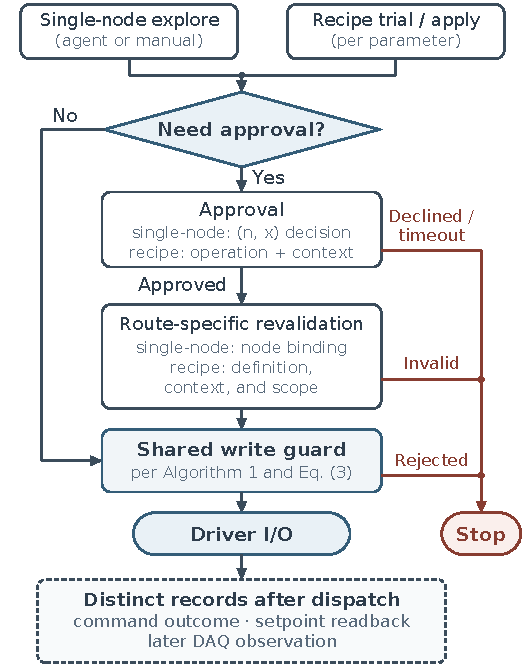
\includegraphics[width=\columnwidth]{resources/fig4-governed-flow.pdf}
\caption{Governed write routes. Both routes reach the write guard but select limits differently. Algorithm~1 and Eq.~(\ref{eq:admission}) describe the online single-node path, not recipe application. Skipping approval does not skip dispatch authorization or write checks. A failed pre-dispatch check stops the affected operation or parameter; recipe writes are not an atomic batch. Driver outcomes, optional readbacks, and later observations are distinct records.}
\label{fig:hitl}
\end{figure}
Fig.~\ref{fig:hitl} maps both write routes onto the shared write guard and the distinct records returned after dispatch; Algorithm~1 details the single-node check sequence. For a manual single-node \texttt{optimization\_explore} request, approval covers the node, proposed value, current effective interval, and rationale; the same boundary receives an agent's typed intent after acquisition and analysis. As in Algorithm~1, a decline or timeout stops the request. Approval triggers revalidation of the original direct node binding or, for recipes, the recipe binding and parameter membership. Single-node approval does not use the recipe-operation context snapshot described next. In either path, revalidation does not make the checks and the external device write atomic.

For \texttt{recipe\_trial} and \texttt{recipe\_apply}, approval is bound to the recipe operation and
active line--product--recipe--run context. After approval, the handler checks
authority and context again and verifies the recipe definition and
candidate scope before dispatch. A changed context, revoked binding, or
changed recipe definition prevents that proposal from proceeding. Recipe-trial approvals default to a 30-minute window; single-node approval waits expire after 180\,s. Outside benchmark mode, writes require a minimum 60-s interval after a setpoint change, and recipe trials a per-line cadence of 300~s.

A \texttt{recipe\_trial} submits a bounded batch from the agent's control intent through the configured driver and returns a result per parameter to the calling route. Parameters are attempted individually, so a batch can be partially applied; results and device state must be reconciled before any retry. A trial neither saves nor applies a recipe version; later DAQ observations can be retrieved separately before updating, applying, or rolling back the recipe.

As sketched in Fig.~\ref{fig:hitl}, receipts record the command outcome returned to the agent or caller, while observations record what followed in the process; results are graded readback-verified, transport-acknowledged, or unverified. For a successful recipe write not already readback-verified, the service may by default attempt up to three additional reads at 2\,s intervals where supported; recipe batches retain per-parameter verification outcomes. A readback-verified result means the returned value matched the request within the applicable tolerance; a transport acknowledgment alone does not establish that the device applied the value, and an unverified result does not establish a matching readback. DAQ stores later timestamped observations for the agent's next analysis turn, while recipe history, approvals, and task records remain with their owning services; identifiers and timestamps can link these records when available, but a later observation alone does not prove that the command caused the measured change.

